\pgfplotsset{
	label style={font=\footnotesize},
	legend style={font=\footnotesize},
	every tick label/.append style={font=\tiny},
        every node near coord/.style={font=\tiny},
        every axis plot/.append style={line width = 0.6pt}
}



\begin{figure}[!ht]
    \centering
\begin{tikzpicture}
%%% ALL
\begin{axis}[
	xlabel=Recall,
        xticklabel pos=right,
	ylabel=Precision,
%	ymin=0,
	ymax=1,
        xmin=0,
        xmax=1,
	%ytick distance=.1,
%	height=0.25\textheight,
	width=0.33\textwidth,
	axis lines=left,
	%% legend entries={RnnOIE,OpenIE-4,PropS,ClausIE},
	%% legend style={draw=none,font=\tiny,at={(1,0.01)}, anchor=south east},
         /pgf/number format/.cd,
        1000 sep={}
]
\addplot[color1,mark size=0pt] table [x=Recall,y=Precision] {../../evaluations/figures/joint/RnnOIE.dat} node[right,pos=1] {\tiny RnnOIE};
\addplot[color2,mark size=0pt] table [x=Recall,y=Precision] {../../evaluations/figures/joint/OpenIE-4.dat} node[left,pos=1] {\tiny OpenIE-4};
\addplot[color3,mark size=0pt] table [x=Recall,y=Precision] {../../evaluations/figures/joint/PropS.dat} node[below,pos=0.7] {\tiny PropS};
\addplot[color4,mark size=0pt] table [x=Recall,y=Precision] {../../evaluations/figures/joint/ClausIE.dat} node[above,pos=1] {\tiny ClausIE};
\end{axis}
\end{tikzpicture}
%% \renewcommand{\thesubfigure}{a}
%% \subfloat[\small{Full Open-IE: PR and AUC.}]{
%% \label{fig:prop}
    \begin{tikzpicture}
  \begin{axis}[
  width = 0.4\textwidth,
  height=5cm,
  xbar,
  xmax = 0.49,
  bar width=2pt,
  xtick= \empty,
  ytick=data,% crucial line for the xticklabels directive
   yticklabels from table={../../evaluations/figures/joint/auc.dat}{system},
nodes near coords,
nodes near coords align={horizontal}
  ]
        \addplot[draw=blue,fill=blue!80!white,mark size=0pt] table [x=auc, y expr=\coordindex] {../../evaluations/figures/joint/auc.dat};
  \end{axis}
\end{tikzpicture}
%% $\;$
%% \renewcommand{\thesubfigure}{b}
%% \subfloat[\small{Predicate extraction: PR and AUC.}]{
%% \label{fig:pred}
%%     \begin{tikzpicture}
%%   \begin{axis}[
%%   width = 0.3\textwidth,
%%   height=3cm,
%%   xbar,
%%   xmax = 0.62,
%%   bar width=2pt,
%%   ytick=data,% crucial line for the xticklabels directive
%%    yticklabels from table={../evaluations/figures/joint/predicate/auc.dat}{system},
%% nodes near coords,
%% nodes near coords align={horizontal}
%%   ]
%%         \addplot[draw=blue,fill=blue!80!white,mark size=0pt] table [x=auc, y expr=\coordindex] {../evaluations/figures/joint/predicate/auc.dat};
%%   \end{axis}
%% \end{tikzpicture}

%%     }
%%     $\;$
%% \renewcommand{\thesubfigure}{c}
%% \subfloat[\small{Argument extraction: PR and AUC.}]{
%% \label{fig:arg}
%%     \begin{tikzpicture}
%%   \begin{axis}[
%%   width = 0.3\textwidth,
%%   height=3cm,
%%   xbar,
%%   xmax = 0.71,
%%   bar width=2pt,
%%   ytick=data,% crucial line for the xticklabels directive
%%    yticklabels from table={../evaluations/figures/joint/arguments/auc.dat}{system},
%% nodes near coords,
%% nodes near coords align={horizontal}
%%   ]
%%         \addplot[draw=blue,fill=blue!80!white,mark size=0pt] table [x=auc, y expr=\coordindex] {../evaluations/figures/joint/arguments/auc.dat};
%%   \end{axis}
%% \end{tikzpicture}
%% }
%%     %% \qquad
%%     %% \subfloat[Figura 3]{
%%     %%     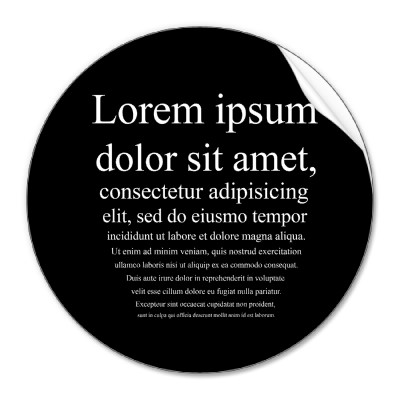
\includegraphics[width=0.4\columnwidth]{./figures/lorem-ipsum.jpg}
%%     %% }
%%     \caption{Precision-recall curves of the different systems on Open IE's subtasks (top),
%%     and corresponding areas under the curve (bottom)  -- complete Open IE (predicate-argument extraction) (\ref{fig:prop}),
%%     predicate extraction (\ref{fig:pred}), and argument extraction (\ref{fig:arg}).
%%     See details in Section \ref{sec:analysis}.
%%     }
%%     \label{fig:subfigname}
\end{figure}


